% ===================================================================
\section{Portal Architecture and Controller Governance}
% ===================================================================

\subsection{The Portal as Semantic Proxy Archive}

The central architectural proposal of this paper is that all \DPP\ data --- including product data originally provided by the Responsible Economic Operator (REO) --- is stored and maintained \textit{behind a federated portal}, rather than at distributed \ERO\ endpoints. The portal acts as a \textbf{semantic proxy archive}: a federation of per-member-state triple-stores --- one per \EU\ member state --- that collectively ingest, validate, store, and serve \DPP\ data as \RDF\ named graphs. Each national instance behaves identically in terms of \API, data model, and access governance, while operating on the data relevant to economic operators registered in that jurisdiction. Figure~\ref{fig:app-mech} provides a conceptual overview of the full architecture, showing the relationships between the federated repository, the ontologised regulations and \SHACL\ brick library, the federated controller and portal, and the tailored app generation pipeline.

\begin{figure}[htbp]
\centering
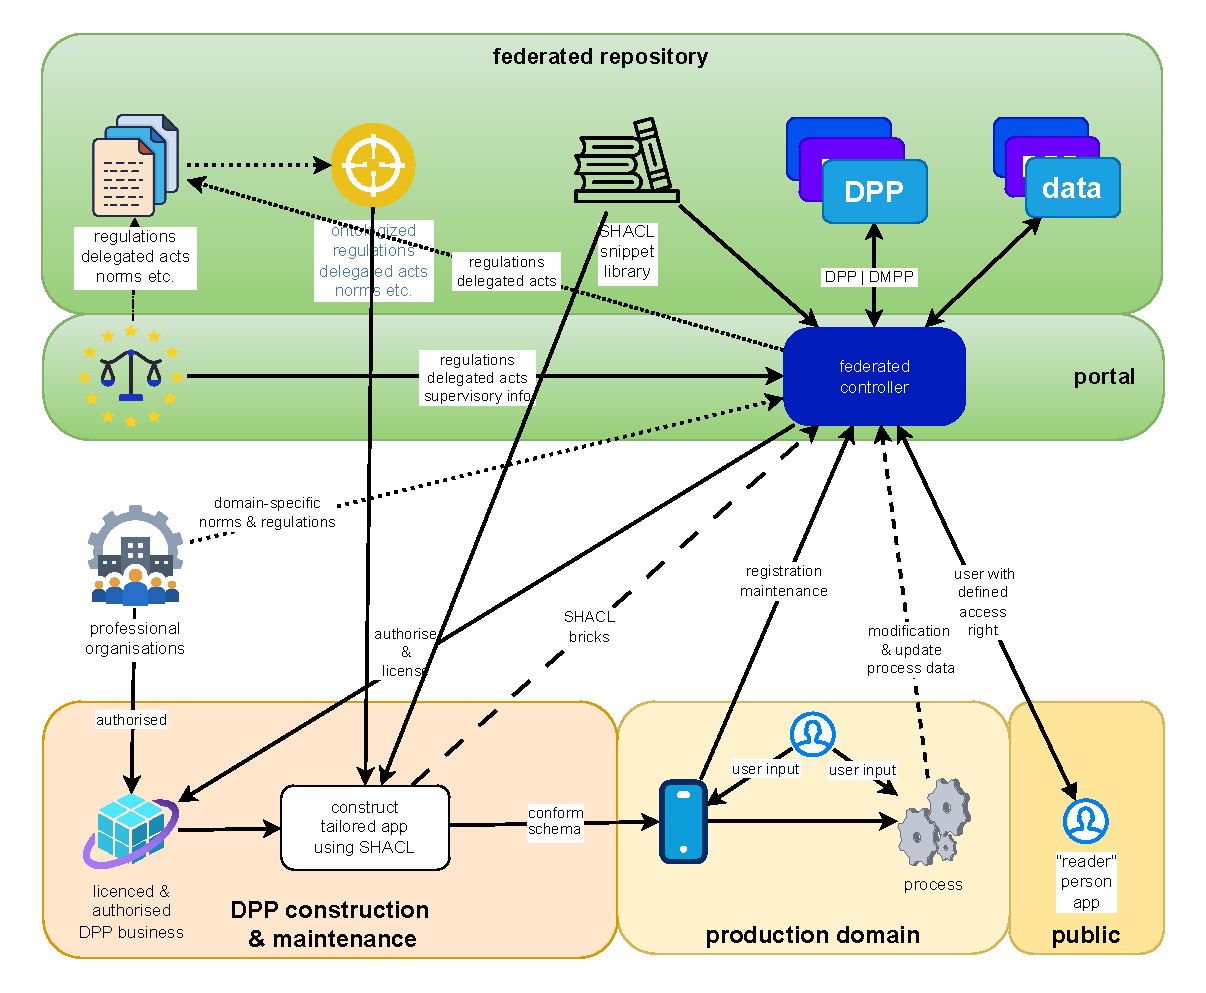
\includegraphics[width=0.9\linewidth]{figures/2025-10-16__DigiPass_DPP_handling-App-mech.pdf}
\caption{Conceptual overview of the portal-backed \DPP\ architecture. The federated repository (top) stores \DPP\ data, ontologised regulations, delegated acts, norms, and supervisory information. Professional organisations authorise and license \SHACL\ bricks, which are assembled into schemas for tailored app generation. The federated controller and portal (centre) govern access, modification rights, and updates. Licensed \DPP\ businesses construct tailored applications from the \SHACL\ schemas, ensuring that user-entered data conforms to regulations by construction. The ``reader'' person app provides public access to \DPP\ data.}
\label{fig:app-mech}
\end{figure}

This design places the responsibility for sustainable, long-term data custody with a clearly identifiable entity per jurisdiction --- the national portal operator --- rather than dispersing it across hundreds of thousands of \EROs\ whose operational continuity cannot be guaranteed over the decades-long lifespan envisioned for \DPP\ data. Each national portal instance is not merely a registry that maps identifiers to external endpoints; it is the authoritative repository of the \DPP\ data for economic operators registered in that jurisdiction. The \EC\ central registry, whose implementing act was identified by the European Commission representative at \DPPforEU~2026 as the first piece of legislation to be adopted~\cite{dpp4eu2026_day1}, provides the identifier resolution and regulatory framework, while the portal provides the data storage and governance layer. The two are complementary: the registry points to the portal, and the portal serves the data.

\subsection{Federation of National Portals}

The federated portal model envisions one portal per \EU\ member state, each behaving identically in terms of \API, data model, and access governance, but operating on data relevant to economic operators registered in that jurisdiction. Thus, the portal is not a single central server: it is a federation of interoperable national portals, each storing and governing the \DPP\ data of economic operators registered in its jurisdiction. This federation addresses sovereignty concerns while maintaining architectural uniformity. A common portal specification provides a unified architectural baseline that proactively addresses the emergence of parallel approaches across jurisdictions, as called for by a JTC~24 conference participant.

\subsection{The Ingestion Governance Loop}

When an \REO\ submits \DPP\ data to the portal, the data passes through an \textbf{Ingestion Governance Loop} --- a sequence of validation, normalisation, and storage operations performed by the portal controller before the data is committed to the triple-store. This loop ensures that all ingested \DPPs\ are semantically valid, cryptographically authenticated, and normalised to canonical ontological entities before they become queryable.

\subsubsection{SHACL Validation}

The first stage of ingestion is validation against \SHACL\ shapes. \SHACL\ (Shapes Constraint Language) is a W3C standard for describing and validating \RDF\ graphs against a set of structural constraints called ``shapes.'' The portal controller maintains a library of \SHACL\ shapes --- one set for each product category and applicable regulation --- and validates every submitted \DPP\ against the shapes corresponding to its product type and regulatory context. If validation fails, the \DPP\ is rejected with a structured error report indicating which shapes were violated and which data points failed. 
This design directly addresses the conference observation that machine-readable product data must become checkable by machine-readable regulation (see Section~6.2 for a detailed discussion of \SHACL\ conformity checking).
The portal-backed architecture makes this a present capability by hosting both the \DPP\ data and the \SHACL\ validation shapes in a unified triple-store within each national portal instance, enabling automated compliance checking at ingestion time.

\subsubsection{Cryptographic Alignment}

Each submitted \DPP\ must be cryptographically signed by the \REO\ that authored it. The portal controller verifies the signature against the \REO's registered public key, which is bound to the \REO's identity through the trust tier matrix (Section~5). This ensures that only authenticated, authorised economic operators can submit \DPP\ data to the portal. The cryptographic signature also provides non-repudiation: once a \DPP\ is submitted and signed, the \REO\ cannot deny authorship of the data. While the conference discussion on data carrier verification focused on verifying the physical carrier (e.g., \QR\ code on a product)~\cite{dpp4eu2026_day1}, the portal-backed architecture extends verification to the data layer itself: every \DPP\ in the triple-store is cryptographically authenticated.

\subsubsection{External Entity Normalisation}

\DPP\ data frequently references external entities: chemical substances (identified by \CAS\ numbers or \EC\ numbers), standards (identified by standard numbers), certifiers (identified by accreditation body identifiers), and materials (identified by various classification schemes). The portal controller normalises these references to canonical \IRIs\ using a set of external registry lookup services. For example, a reference to a chemical substance submitted as ``CAS 7440-44-0'' is normalised to a canonical \IRI\ such as \texttt{urn:echa:substance:7440-44-0}, linking it to the \ECHA\ database entry for that substance. This normalisation ensures that all \DPPs\ in the triple-store use consistent, resolvable identifiers for external entities, enabling cross-\DPP\ queries (e.g., ``find all products containing this substance'') to execute correctly. This design is grounded in the conference observation that the \DPP\ must link to standards, measurements, and certificates through the quality infrastructure~\cite{dpp4eu2026_day1}.

\subsection{The Resolution Governance Loop}

When a user (consumer, professional, circular operator, or authority) requests \DPP\ data from the portal, the request passes through a \textbf{Resolution Governance Loop} --- a sequence of authentication, authorisation, graph slicing, and serialisation operations performed by the portal controller before the data is returned to the requester. This loop ensures that each user sees only the data branches they are authorised to access.

\subsubsection{Authentication and Authorisation}

The requester is first authenticated via the \EC\ Authorisation App (Section~5.6), which leverages \eIDAS~2.0 digital identity wallets to establish the requester's identity. The requester's attributes (user category, jurisdiction, organisational affiliation, certifications) are then evaluated against the \ODRL\ access policies attached to each branch of the requested \DPP. This step implements the \ABAC\ framework described in Section~5. The conference observation from the battery passport context --- that the actor should see only ``\textit{those data that he's allowed to see but nothing more}''~\cite{dpp4eu2026_day2} --- is precisely the behaviour implemented by this stage.

\subsubsection{Graph Slicing via Dynamic \SPARQL\ CONSTRUCT}

Once the requester's access rights are determined, the portal controller constructs a \textbf{filtered sub-graph} of the requested \DPP\ --- a view that contains only the data branches the requester is authorised to see. This is implemented as a dynamic \SPARQL\ \texttt{CONSTRUCT} query: the controller generates a query that traverses the \DPP's named graph, selects only the triples whose attached \ODRL\ policies permit access for the requester's attributes, and constructs a new \RDF\ graph containing only the authorised triples. The resulting filtered graph is then serialised in the requested format (\JSONLD, \TURTLE, \RDF/ \XML) and returned to the requester. This approach --- dynamic, query-time filtering rather than pre-computed views --- ensures that access policies can be updated without regenerating stored views, and that the most current policy is always applied.

\subsubsection{Link Traversal Within the Portal}

When the filtered \DPP\ is returned to the requester, it may contain \texttt{dpp:hasPrecursor} and \texttt{dpp:derivedFrom} links to other \DPPs\ within the portal. The requester may then request those linked \DPPs, which pass through the same Resolution Governance Loop. Critically, because all linked \DPPs\ reside within the same portal triple-store, link traversal never produces \texttt{404 Not Found} errors (unless a \DPP\ has been explicitly revoked). The link rot problem --- identified in Section~2 as a systemic risk of the distributed model --- is structurally eliminated. This architectural design directly answers the data persistency concern raised in Section~2.1: data persists because it is stored in a governed repository, not at an unmanaged endpoint.

\subsection{Relationship to the \EC\ Central Registry}

The portal-backed architecture is complementary to, not competitive with, the \EC\ central registry. The registry provides:

\begin{itemize}
\item \textbf{Identifier resolution}: mapping product unique identifiers (as defined in EN~18215 \cite{en18215}) to portal endpoints.
\item \textbf{Regulatory metadata}: hosting the \SHACL\ shape library and ontologised regulations (Section~6).
\item \textbf{Public key infrastructure}: registering \REO\ public keys for cryptographic verification.
\item \textbf{Audit and compliance}: logging portal operations for regulatory oversight.
\end{itemize}

The portal provides:

\begin{itemize}
\item \textbf{Data storage}: hosting \DPP\ named graphs in a per-member-state triple-store.
\item \textbf{Ingestion governance}: \SHACL\ validation, cryptographic alignment, entity normalisation.
\item \textbf{Resolution governance}: \ABAC-based graph slicing, \SPARQL\ CONSTRUCT filtering.
\item \textbf{Link traversal}: resolving \texttt{dpp:hasPrecursor} and \texttt{dpp:derivedFrom} within the portal.
\end{itemize}

This division of responsibility resolves the tension observed at \DPPforEU~2026, where the Materials Commons initiative acknowledged that it does not ``\textit{run servers in the end}''~\cite{dpp4eu2026_day2}. The portal-backed architecture fills this gap: it runs the servers, stores the data, and governs access, while the \EC\ central registry provides the identifier, regulatory, and oversight layer.

\subsection{The Public Repository for Ontologised Regulations and Standards}

A critical component of the portal architecture is a \textbf{public repository 
for ontologised regulations and standards}, hosted on the \EC\ \DPP\ registry 
alongside the \SHACL\ shape library. This repository contains machine-readable 
representations of legal requirements, delegated acts, and harmonised 
standards that apply to each product category. The conference principle that 
``\textit{everything needs to be ontologized}''~\cite{dpp4eu2026_day2} is 
realised through this repository: regulations, standards, data models, and 
validation shapes are all represented as semantic, machine-readable artefacts 
within a unified framework. Section~6 discusses the public repository, the 
\SHACL\ brick library, and the two-stage design toolchain in detail.


\subsection{The Portal \API}

The portal exposes a standardised \REST\ \API\ that enables economic operators and application developers to interact with the portal controller programmatically. As a conference participant emphasised at \DPPforEU~2026~\cite{dpp4eu2026_day1}, the \API\ should cover ``\textit{all major business cases of registering... first of creating a digital product passport, being able to update it being able to delete or revoke it and then finally to register it with the European Commission's \DPP\ registry}''. A standardised \API\ is essential because, as another participant observed~\cite{dpp4eu2026_day1}, ``\textit{the implementation of an \API\ creates no unique selling point for anyone}'' and leaving \API\ implementation to small teams is ``\textit{already too much for them}''. The portal \API\ aligns with the \JTC~24 \API\ module (EN~18222~\cite{en18222}) and the Asset Administration Shell \API\ specifications~\cite{dpp4eu2026_day1}, which are ``\textit{already in review and publicly accessible}''~\cite{dpp4eu2026_day2}.

The portal \API\ is organised around five operation groups corresponding to the \DPP\ lifecycle:

\begin{enumerate}
\item \textbf{Authentication}: The requester presents an \eIDAS~2.0 digital identity credential to the \EC\ Authorisation App (Section~5.6), which returns a short-lived bearer token containing the requester's attributes (user category, organisation, jurisdiction, certifications).
\item \textbf{\DPP\ Lifecycle Management}: Authenticated \REOs\ can create, read, update, revoke, and register \DPPs. Each operation passes through the Ingestion Governance Loop (Section~4.2) for \SHACL\ validation, cryptographic alignment, and external entity normalisation before the \DPP\ is committed to the triple-store.
\item \textbf{\DPP\ Resolution}: Authenticated users can request a \DPP\ by its unique identifier. The request passes through the Resolution Governance Loop (Section~4.3), which evaluates \ODRL\ policies against the requester's attributes and returns a filtered sub-graph containing only the authorised branches.
\item \textbf{Link Traversal}: Authenticated users can request linked \DPPs\ by following \texttt{dpp:hasPrecursor} and \texttt{dpp:derivedFrom} links returned in a resolved \DPP. Each linked \DPP\ request passes through the same Resolution Governance Loop.
\item \textbf{\SPARQL\ Query}: Advanced users (professional users, circular operators, market surveillance authorities) can submit \SPARQL\ queries against the portal's triple-store. The portal controller executes the query with dynamic \ODRL-based graph filtering, returning only triples from branches the requester is authorised to access.
\end{enumerate}

The full \API\ specification, including endpoint paths, \HTTP\ methods, request and response schemas, and authentication flows, is provided in Appendix~\ref{app:api-spec}. Example interaction sequences covering the five operation groups are provided in Appendix~\ref{app:api-examples}.
